\documentclass[11pt]{article}

\usepackage{graphicx}
\usepackage{amsmath}
\usepackage[margin=0.8in]{geometry}
\usepackage{float}


\usepackage{listings}
\usepackage{xcolor}

\definecolor{codegreen}{rgb}{0,0.6,0}
\definecolor{codegray}{rgb}{0.5,0.5,0.5}
\definecolor{codepurple}{rgb}{0.58,0,0.82}
\definecolor{backcolour}{rgb}{0.95,0.95,0.92}

\lstdefinestyle{mystyle}{
	backgroundcolor=\color{backcolour},   
	commentstyle=\color{codegreen},
	keywordstyle=\color{magenta},
	numberstyle=\tiny\color{codegray},
	stringstyle=\color{codepurple},
	basicstyle=\ttfamily\footnotesize,
	breakatwhitespace=false,         
	breaklines=true,                 
	captionpos=b,                    
	keepspaces=true,                 
	numbers=left,                    
	numbersep=5pt,                  
	showspaces=false,                
	showstringspaces=false,
	showtabs=false,                  
	tabsize=2
}

\usepackage{tikz}
\usetikzlibrary{shapes.geometric, arrows}
\tikzstyle{startstop} = [rectangle, rounded corners, minimum width=3cm, minimum height=1cm,text centered, draw=black, fill=red!30]
\tikzstyle{io} = [trapezium, trapezium left angle=70, trapezium right angle=110, minimum width=3cm, minimum height=1cm, text centered, draw=black, fill=blue!30]
\tikzstyle{process} = [rectangle, minimum width=3cm, minimum height=1cm, text centered, draw=black, fill=orange!30]
\tikzstyle{decision} = [circle, text centered, draw=black, fill=green!30]
\tikzstyle{arrow} = [thick,->,>=stealth]


\lstset{style=mystyle}

\title{MECH 423 Final Project Proposal\\
		The No Excuses Waking Up System}
\author{Dana Deutsch\\
		deutschdana@gmail.com}
\date{November 1st 2020}
\begin{document}
\maketitle
\newpage
\tableofcontents
\newpage

\section{Objectives}
The goal of this project is to create an alarm clock system for people who have a hard time waking up and getting out of bed.
Many people simply turn off their alarms and fall back asleep.
Then they must to set multiple alarms at various intervals to remind themselves to get up.
This is a temporary solution since you can still turn off all the alarm and stay in bed.
My objective of my system is to eliminate the possibility of remaining in bed by taking away the power to fully "turn off" the alarm while keeping a short "snooze" functionality. 
The reason for the snooze is because people enjoy laying in bed for a few minutes before fully waking up and a consistent alarm while in bed will get annoying. 
Since most people don't use a physical alarm clock and instead use their phones, this system will work best if it were to interface with the phone people already use.\\

Creating a phone application interface is outside the scope of this project as it adds a lot much functions and complexity for the short timeline provided. 
Instead the goal of the project is to use the phone alarm sound as a trigger point for an bed detecting alarm system which operates separate from the phone,
This way the main alarm can be set on the phone which users already have set up since it has a better interface and more alarm features.
However , the device run on the a microcontroller still operates in respect to the phone. 
The device will sense when the phone alarm goes off in order to begin its functions instead of having its own internal real time clock and alarm setting capacity.  
After the original alarm, the device will periodically ring after the user "snoozes" until the user leaves the bed and doesn't return to bed for a set amount of time. 
The device will look like a small box that is placed by the bed right where the user normally places their phone to charge.
The device will have small wires leading to sensors under the bed to connect to the detection circuitry.

\section{Rationale}
I want to make this device since it solves a problem I face daily along with many other people.
Instead of setting up 5 different alarms which are close together and spread out to make sure I get up, I can use this device.
I sometimes ignore my alarms and just decide to keep sleeping so this way I will be forced to get up and hopefully fix my sleeping scheduled.
This product isn't available on the market right so its only achievable by making it myself.
I hope this project will provide a concept functionality prototype for a possible market device that uses this method or a better phone app interface. 
As well many home automation can be made using the bed occupancy detection function like starting the coffee maker when you leave the bed.
An example of how I imagine a final product to look like is found in Figure \ref{fig:market}.

\begin{figure}[H]
	\centering
	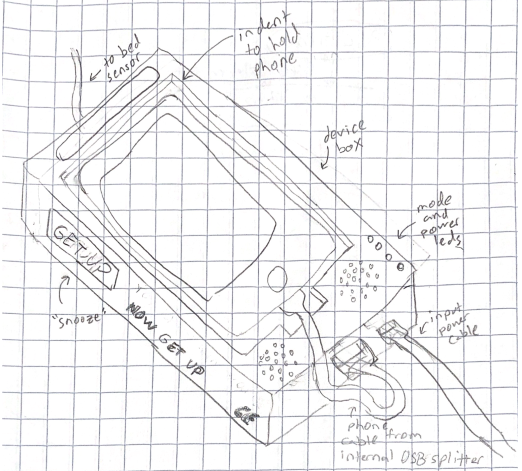
\includegraphics[width = 0.5\linewidth]{marketSolution}
	\caption{Concept Drawing For a Alternative Version of the Device Integrated in a Phone Charging Station}
	\label{fig:market}
\end{figure}

\section{Functions}
The functional requirements are found in Table \ref{tab:FR}.
The hardware components include the microcontroller (MCU), a input force sensor for the bed, input audio sensor circuitry for detecting the phone alarm, and output buzzer to create its own alarm sounds. 
The MCU is used to to control the logic for when the alarm are rung and when to detect and control the inputs and outputs.
The MCU code must read the output of the force and sound sensor to detect if the user is in bed or if the phone has rung based on calibration values.
The MCU also sends an output signal to play a buzzer for the alarm sounds. \\

I created a few requirements for the functions ordered by importance.
The MCU alarm ringing code cannot be tricked to stop its detection logic.
The bed sensor must be able to consistently detect the user regardless of their position in bed.
The detection of the user must also be integrated without compromising the bed comfort or permanently changing the bed structure.
The buzzer must be laud enough to wake a person from a light sleep.
Since deep sleep wont be achievable in the "snooze time", the phone alarm will be the main sound that will wake the user.
Lastly the sound detection shouldn't get accidentally triggered by a person talking while on the bed.\\

\begin{table}[H]
	\centering
	\caption{Functional Requirements for The Wake Up System}
	\begin{tabular}{|l|l|l|}
		\hline
		&\textbf{Functions} & \textbf{\% Effort} \\
		\hline
		1&Bed Occupancy Detection (Circuitry and Calibration Code) & 50\\
		2&MCU Alarm Control Code &30\\
		3&Phone Audio Detection and Output (Circuit and Code)& 20\\
		\hline
	\end{tabular}
	\label{tab:FR}
\end{table}

\section{Bed Occupancy Detection Circuitry and Calibration}
\subsection*{Approach and Design}
For the bed detection circuitry I research possible solution and found two solutions for sensors that should work by looking at online projects. 
The first used half-bridge load cells, particularly the types found in bathroom scales. 
The second method uses thin film force sensitive resistors (FSR) which are created based on a material which changes it's resistance due to being pinched and flexed. 
I had also considered off the shelf products which are expensive.
The only market product I found which almost meets this function is a bed detection mat for the elderly which are used to see if the user has fell, and alert a special service to come help them.  
I plan to first try the half bridge strain gauges load cell solution and if it doesn't work I have the FSR solution as backup.
The reason for choosing the load cells instead of the FSR are found in this section and Table \ref{tab:solutionComparison} summarizes this comparison. 
Apart from the circuitry the solution will also need  to be calibrated to determine values for when the code considers the bed occupied or not.
\\

A bathroom scale has four force sensors at the corners which are actually strain gauged sheet metal parts.
Each sensor is a half bridge with each side having opposites effects from compression and tension. 
I plan to purchase a set from amazon from 13\$ which also comes with a 24 bit Analog to Digital Converter (ADC) and amplifier , HX711, pictured in figure \ref{fig:loadcellproduct}. 
To measures the weight we position the strain gauges in a Wheatstone bridge circuit. 
The HX711 then amplifies the signal across the bridge and converts it to a 24 bit digital signal to provide precision.
These sensors are commonly used to create scales using an Arduio therefore there is a lot of online documentation and libraries I can read and adapt on configuring them to the MSP430. 
In figure \ref{fig:Bridge} I show how a Wheatstone bridge interfaces with the ADC module.
In figures \ref{fig:hx711blocks} and \ref{fig:HX711}, I have the block diagram for the HX711 module and Schematic for the board.
The interface for the HX711 is a digital output so to read one 24 bit value I will need to input 25 clock signals and capture the outputs with an MCU code, the process is described in the HX711 data sheet and a small capture is seen in figure \ref{fig:hx711Communication}.\\

Since I don't need to measure the exact weight of the user for this function, only a change is the overall detected weight, I plan to place the sensors at only one or two corners of the bed which should create sufficient detection without capturing the full forces of the bed. 
This makes the device easier to use, install, and over all more adjustable for other beds. 
Another positive aspect of the design is that it doesn't interfere with the mattress or pillow which can make changing the sheets more difficult or reduce user comfort.\\
\begin{figure}[H]
	\centering
	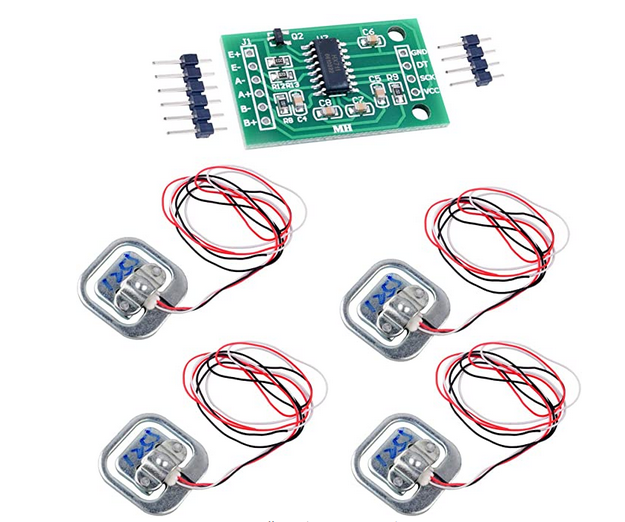
\includegraphics[width = 0.5\linewidth]{Half-bridge-Gagues}
	\caption{The 4 bathroom scale load cells and 24 ADC module}
	\label{fig:loadcellproduct}
\end{figure}
\begin{figure}[H]
	\centering
	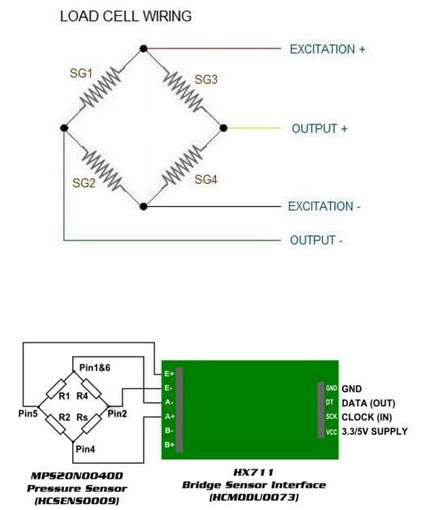
\includegraphics[width = 0.4\linewidth]{bridgeConnefiguration}
	\caption{Measuring Across a Wheatstone Bridge}
	\label{fig:Bridge}
\end{figure}
\begin{figure}[H]
	\centering
	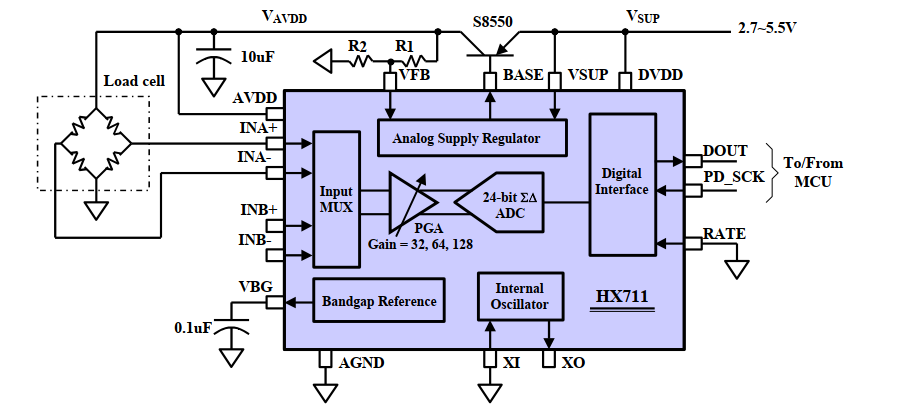
\includegraphics[width = 0.7\linewidth]{hx711applicationBlock}
	\caption{Function Block Diagram for the HX711 Chip}
	\label{fig:hx711blocks}
\end{figure}
\begin{figure}[H]
	\centering
	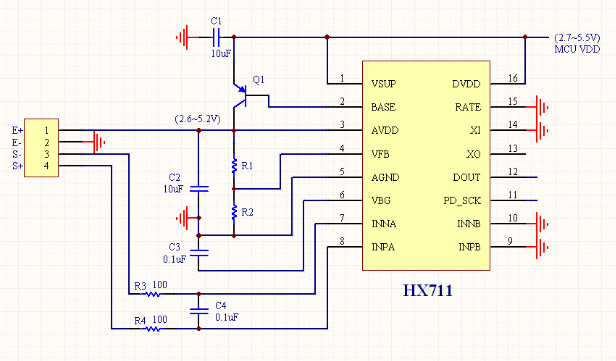
\includegraphics[width = 0.7\linewidth]{HX711}
	\caption{Schematic for the HX711 Load Sensor Board}
	\label{fig:HX711}
\end{figure}
\begin{figure}[H]
	\centering
	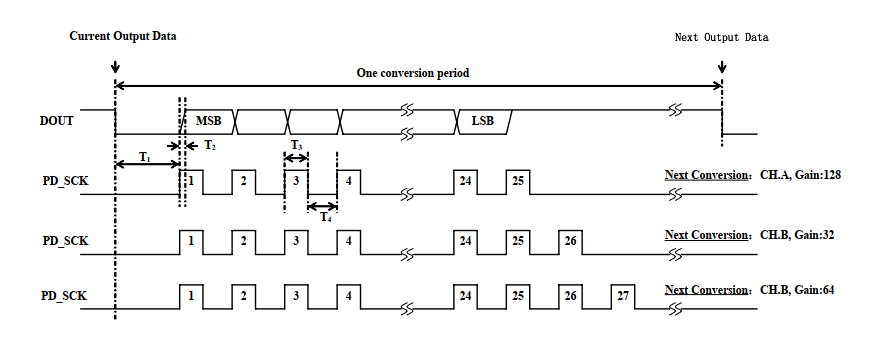
\includegraphics[width = 0.8\linewidth]{exampleDatashaeet}
	\caption{Communication for the HX711 Example from Data Sheet}
	\label{fig:hx711Communication}
\end{figure}
\newpage
From concept testing I devised that placing two sensors under the corner of the bed should be sufficient since each sensor supports up to 50kg. 
The rough measurements I got from my preliminary test was around 32kg appearing at one corner with myself laying on the bed.
I want to include a margin for larger beds as mine is light, other weight users, and safety.
Figure \ref{fig:preliminary} shows my test of an opened bathroom scale with the two gauges removed and placed under one bed leg. 
In this picture I show an empty bed at 15kg under a bed leg. 
The full diagram of the circuit I plan to make is found in figure\ref{fig:loadcellconnetion}.

\begin{figure}[H]
	\centering
	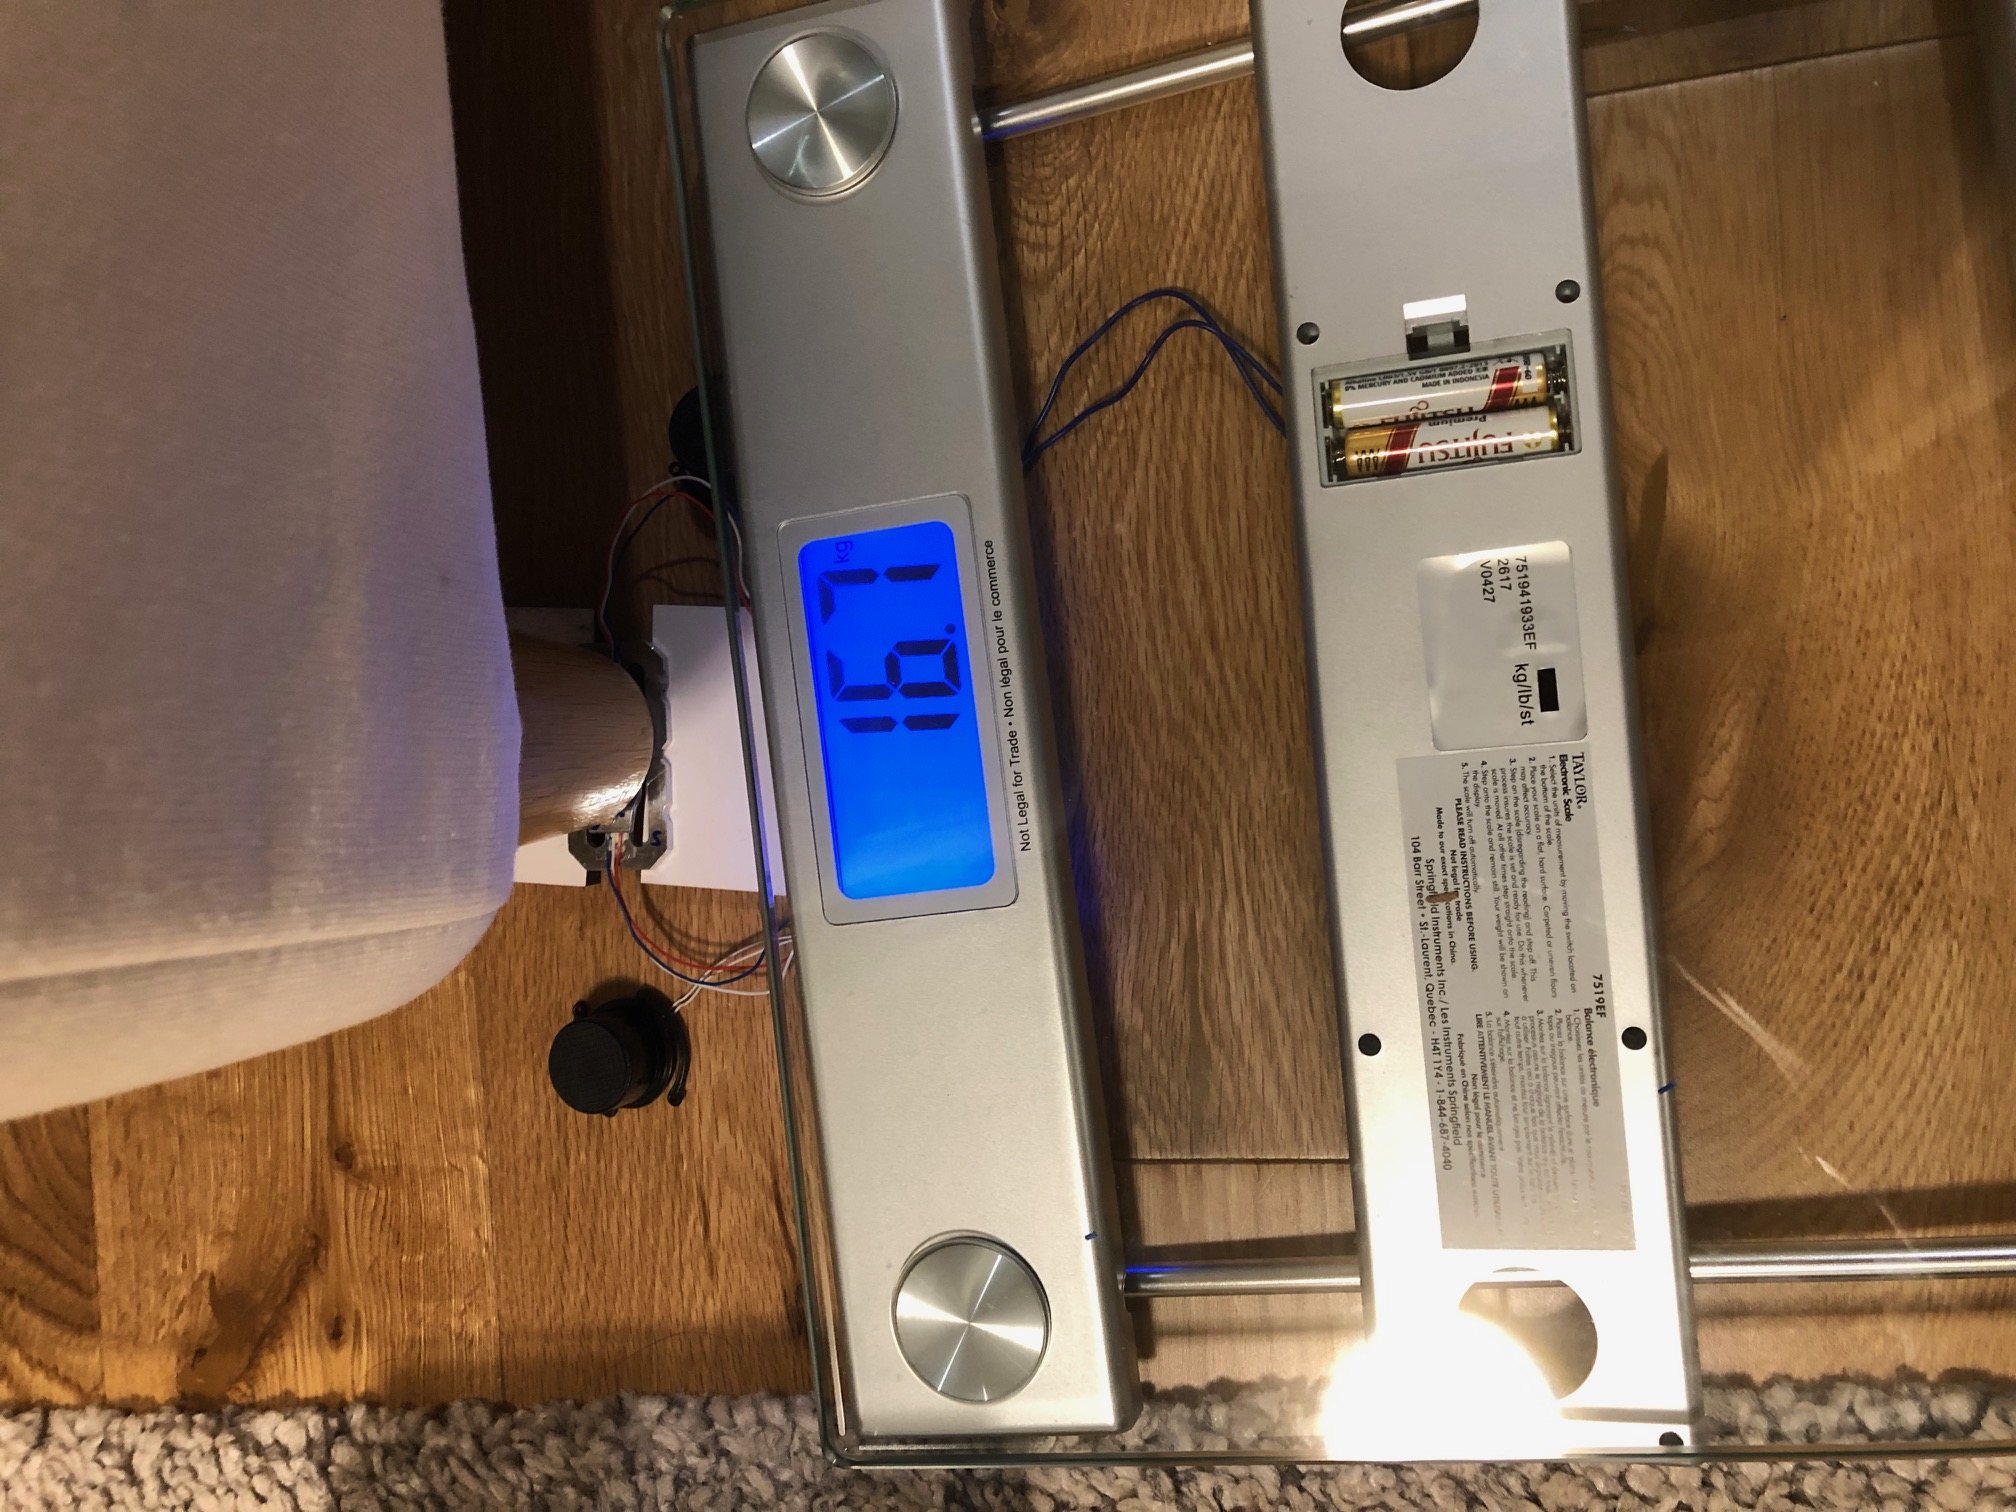
\includegraphics[width = 0.5\linewidth, angle = 270]{preliminarytest}
	\caption{Preliminary Test With Bathroom Scale}
	\label{fig:preliminary}
\end{figure}
\begin{figure}[H]
	\centering
	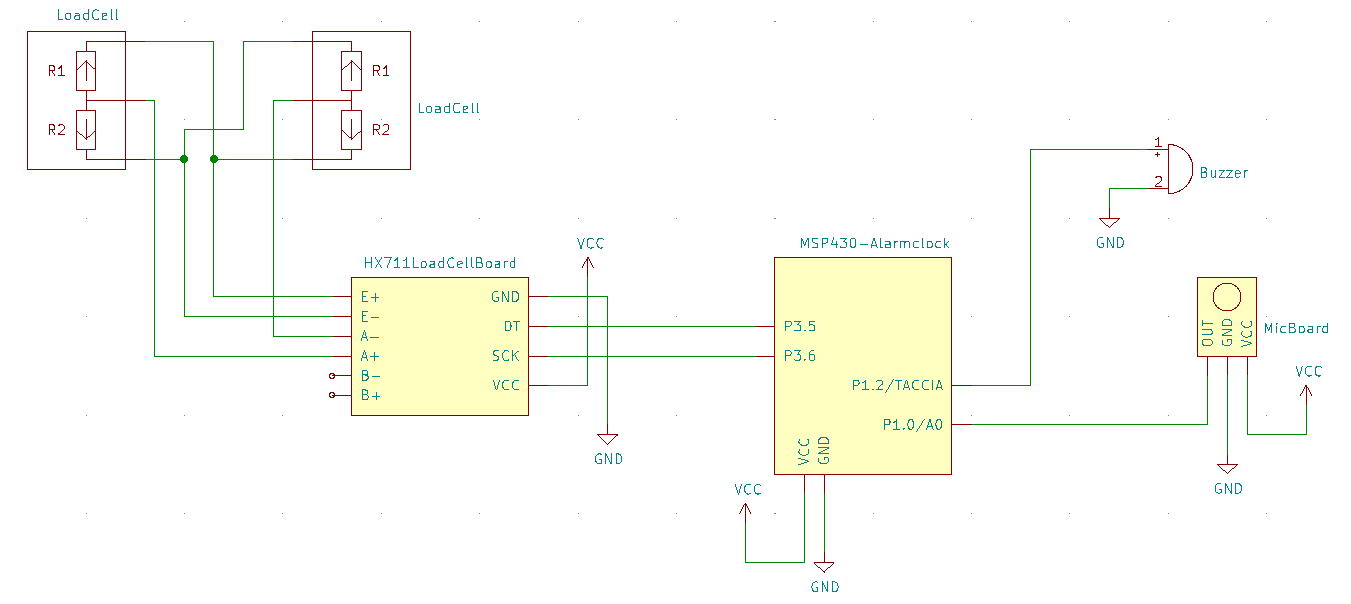
\includegraphics[width = \linewidth]{fullScem}
	\caption{Connection Schematic for The Full Load Cell design}
	\label{fig:loadcellconnetion}
\end{figure}
\newpage
The second solution I am considering as a back up is using force sensitive resistors (FSR).
This thin film resistor reduce their resistance when pinched or flexed. 
I plan to use a long thin resistor which will also detect flex and place it under the mattress on top of the bed slats. 
Other possible locations to mount this resistors also include right under the user head on the pillow, and right under the user upper body on top of the mattress. 
The measured value from this is an analog input into the MCU's ADC. 
However, this solution might cause interference with the bed sheets and might not have enough pressure to provide results.
Also to recognize if the user is on the bed in any position I may need more than one resistor and spread them out on the bed. 
As well different bed frames and mattresses flex a different amount so there is uncertainly if my bed would work.
I have also read that these resistors are fragile and I want the product to be robust and durable with different beds.
For these reasons and those in \ref{tab:solutionComparison}, this will be my backup solution.
Figure \ref{fig:FSR} and figure \ref{fig:FSRScem} show the FSR and how it can be connect to the MCU in a voltage divider. 


\begin{figure}[H]
	\centering
	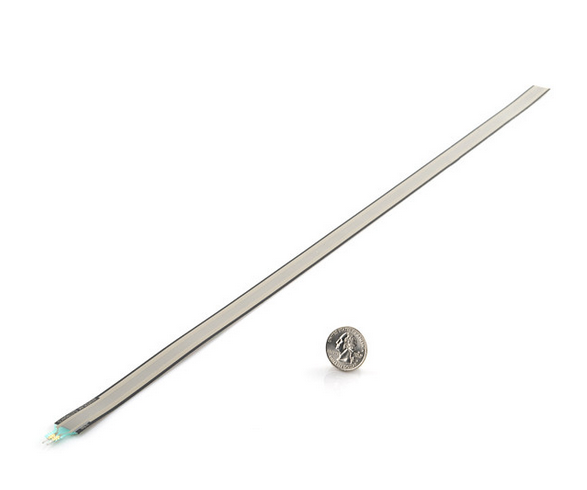
\includegraphics[width = 0.3\linewidth]{FSR}
	\caption{Preliminary test with bathroom scale}
	\label{fig:FSR}
\end{figure}
\begin{figure}[H]
	\centering
	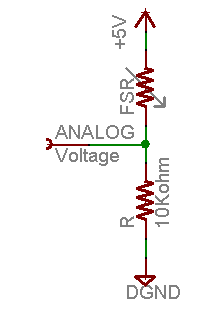
\includegraphics[width = 0.2\linewidth]{FSRscem}
	\caption{Preliminary test with bathroom scale}
	\label{fig:FSRScem}
\end{figure}

\begin{table}[H]
	\centering
	\caption{Comparing the two top bed detecting occupancy solutions}
	\begin{tabular}{|l|l|l|}
		\hline
		Solution & Positives & Negatives \\
		\hline
		Load Cells &	\textbullet  Independent to actual bed structure & \textbullet Each cell max to 50kg \\
								&	\textbullet Worked in online sources& \textbullet More complex electrical setup and integration\\
								&	\textbullet Cheaper & \textbullet Need mechanical holders for the gauges\\
								
		\hline
		FSR & \textbullet Simple circuit and code &\textbullet At least double the cost \\
			& \textbullet No mechanical setup & \textbullet Require positioning around the mattress \\
			&&Could snag wiring from sheets\\
			\hline	
	\end{tabular}
\label{tab:solutionComparison}
\end{table} 

\subsection*{Inputs and Outputs}
The main input to this function is the person providing force by laying on the bed.
As well, we provide the supply voltage VCC from the MCU for the sensor circuit.
The main output is the digital or analog value of the detected voltage.
Each concept has different inputs and outputs seen in the table \ref{concepoutputs}.
The table lists both the output of the circuit and the output from the reading sensor code needed to read the circuit voltage output. 
\begin{table}[H]
	\caption{Output for Bed Detection Concepts}
	\label{concepoutputs}
	\begin{tabular}{|l|l|l|}
		\hline
		Concept & Inputs & Outputs\\
		\hline
		Load Cells & Pulses for reading ADC value& Circuit: Digital value for the voltage from ADC\\
		&VCC & Code: A state variable post calibration value comparison\\ 
		\hline
		FSR &VCC& Circuit: Analog voltage for MCU's ADC10  \\ 
		 & &Code: A state variable post calibration value comparison\\
		 \hline
	\end{tabular}
\end{table}

\subsection*{Parameters}
I will need to power the sensors at Vcc and detect the output value. 
The main parameter is the voltage value which is measured across the changing resistances. 
As well I need need a parameter for calibration of an empty bed and another value as the passing value to signify a person is in bed. 

\subsection*{Development Plan}
I have two development plans, one for each concept. \\

\textbf{Half-Bridge force sensor:}
\begin{itemize}
	\item Connect full bridge detection circuitry using only two force sensors 
	\item Create MCU code to read the digital outputs 
	\item Determine if the change is significant when off and on the bed
	\item Connect 4 force sensors in the bridge at two different corners if needed
	\item Determine calibration values 
\end{itemize}

\textbf{FSR resistor force sensor:}
\begin{itemize}
	\item Connect detection circuitry
	\item Create MCU code to read the ADC values
	\item Determine if the change is significant when off and on the bed by moving around the placement of the resistors to various positions around the bed
	\item Determine calibration values 
\end{itemize}
\subsection*{Test Plan}
To test the user detection I will lay at various locations on the bed and read the outputs.
If the location and position is indeterminate to the final output from the reading code and all pass as the user is in bed than I will consider it a pass. 
An optional test which isn't critical is to place various items like a laptop, laundry basket, and some textbooks on the bed to check the detection isn't too sensitive. 
This test doesn't need to pass since alarm wont be sounding in these cases.

\section{Main MCU Timing Code for Alarms}
\subsection*{Approach and Design}
The MCU is the control behind when the alarms go off based on our hardware inputs. 
The flowchart to the logic behind the alarms are found in figure \ref{fig:flow}.
The code will relay on the use of MCU timers. 
I will be creating this code under assumptions that the inputs will be digital high or low values simulated using IO pins. 
This will be changed when combining this function's MCU code with the code for reading each sensor.
Some features of the flowchart include not ringing the alarm originally if the person isn't in bed but still check they don't return to bed in case they just happen to get up a few minutes before the alarm.
As well if the person returns to bed after exiting, the counter for waiting at least an hour to ensure they don't return will be reset.

\begin{figure}[H]
	\centering
	\label{fig:flow}
	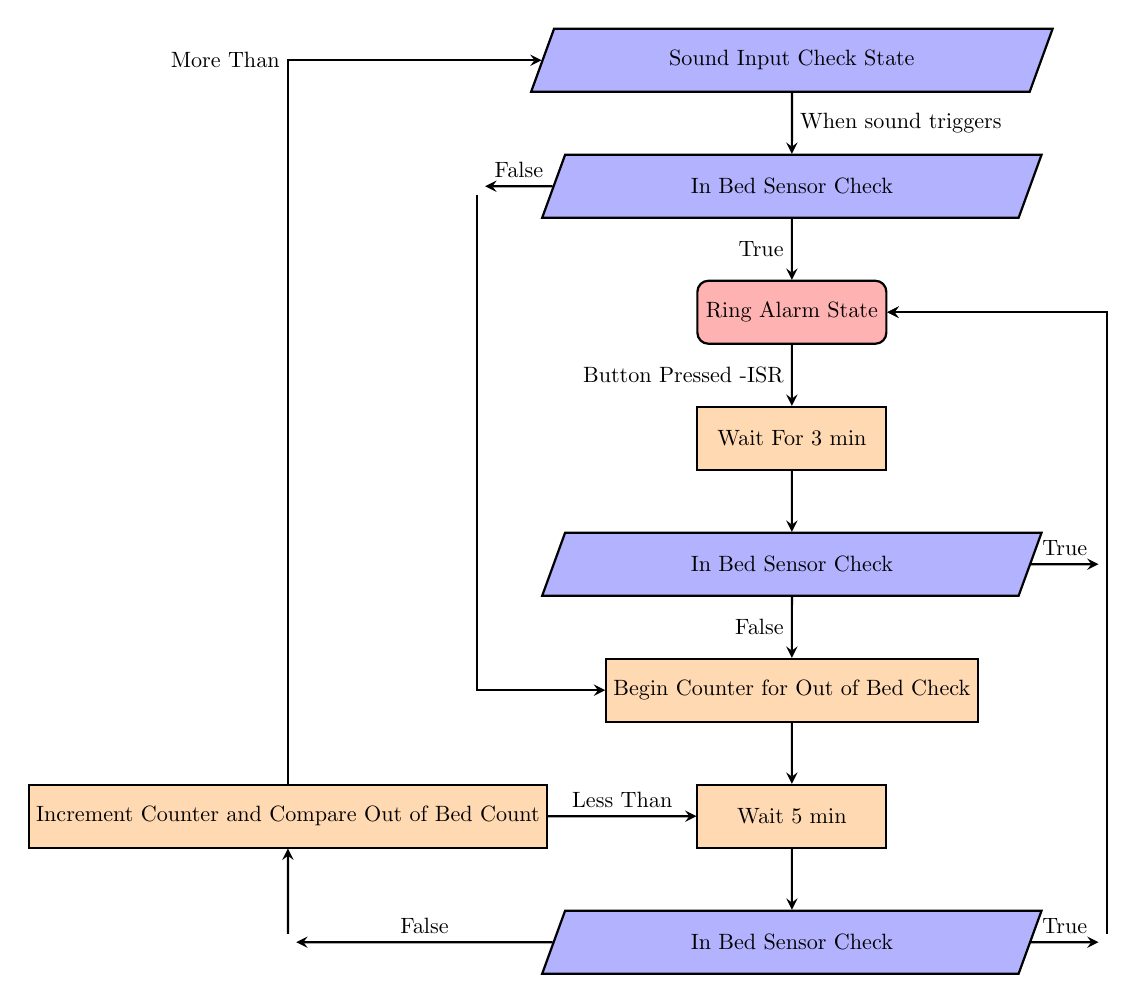
\begin{tikzpicture}[node distance =2cm, thick,scale=0.9, every node/.style={scale=0.8}]
		
		\node (Realtime) [io] {Sound Input Check State}; 
		\node (InBed3) [io, below of=Realtime] {In Bed Sensor Check};
		\node (return2) [left of=InBed3, xshift =-3cm]{}; 	
		\node (Ring1) [startstop, below of =InBed3] {Ring Alarm State};
		\node (Wait1) [process, below of=Ring1] {Wait For 3 min };
		\node (InBed) [io, below of=Wait1] {In Bed Sensor Check}; 
		\node (OutTimer) [process, below of=InBed] {Begin Counter for Out of Bed Check};
		\node (return) [right of=InBed, xshift = 3cm]{};
		\node (wait2) [process, below of=OutTimer] {Wait 5 min};
		\node (InBed2) [io, below of=wait2] {In Bed Sensor Check}; 
		\node (Checkout) [process, left of=wait2, xshift =-6cm] {Increment Counter and Compare Out of Bed Count};
		\node (return1) [right of=InBed2, xshift =3cm]{};
		\node (return3) [left of=InBed2, xshift =-6cm]{};
		
		
		\draw [arrow] (Realtime) -- node[anchor=west] {When sound triggers}(InBed3);
		\draw [arrow] (InBed3) -- node[anchor=east] {True}(Ring1);
		\draw [arrow] (InBed3) -- node[anchor=south] {False}(return2);
		\draw [arrow] (return2) |- (OutTimer);
		\draw [arrow] (Ring1) -- node[anchor=east] {Button Pressed -ISR } (Wait1);
		\draw [arrow] (Wait1) -- (InBed);
		\draw [arrow] (return) |- (Ring1);
		\draw [arrow] (InBed) -- node[anchor=south] {True} (return);
		\draw [arrow] (InBed) -- node[anchor=east] {False} (OutTimer);
		\draw [arrow] (OutTimer) --  (wait2);
		\draw [arrow] (wait2) --  (InBed2);
		\draw [arrow] (InBed2) -- node[anchor=south] {False} (return3);
		\draw [arrow] (InBed2) -- node[anchor=south] {True}(return1);
		\draw [arrow] (return1) |- (Ring1);	
		\draw [arrow] (return3) -- (Checkout);	
		\draw [arrow] (Checkout) -- node[anchor=south] {Less Than}(wait2);
		\draw [arrow] (Checkout) |- node[anchor=east] {More Than}(Realtime);
	\end{tikzpicture}
	\caption{Flowchart for the Alarm Actuation Logic}
\end{figure}

\subsection*{Inputs and Outputs}
The main input is the determined output from the bed occupancy detection. 
This will be a Boolean value to determine if the level passed the allowed amount and the person is in bed. 
The second input is the output from the phone audio sensor which actuates the entire flow chart. 
The third input is a snooze button for the user to temporarily turn off the alarm.
Finally we have the output buzzer to get the user out of bed which will be set with a PWM signal to change frequencies of sound. 
I would also want to include some LEDs for user visual feedback to show if the device is sensing a person in bed and that the device is either idle or in the wake up sequence.  
 
\subsection*{Parameters}
The software will check and use the following to function:
\begin{itemize}
	\item The state of the bed as a digital high or low
	\item The state of the audio volume as a digital high or low 
	\item Count of number of times the secondary alarm has gone off to provide enough time for out of bed detection
	\item Time for waiting between snooze to be converted into frequency of the timer and possibly a count variable is frequency isn't achievable
	\item Time for waiting between checking if the bed is still empty to be converted into frequency of the timer and possibly a count variable is frequency isn't achievable
	\item PWM duty cycle for the piezo buzzer
\end{itemize}

\subsection*{Development Plan}
I will develop this function first independently from the other functions and than merge them. 
Therefore originally the inputs to the system will be simulated before the real inputs are merged.

\begin{itemize}
	\item Develop code for the first half of the flow chart which stops the snoozing loop when user exits bed
	\item Use a buzzer output, snooze push button input, and digital high or low values for the bed and volume detection to test the state machine
	\item Develop the second half of the flow diagram code that checks the our of bed sequence
	\item Test flow again 
	\item Swap the digital inputs for the outputs of the other functions when merging 
\end{itemize}

\subsection*{Test Plan}
Testing on the code will be preformed using test cases based testing of the state machine. 
I will basically pretend to be the user using the simulated inputs.
I will try combinations of "leaving" and "exiting" to test the state machine. 

\section{Phone audio detection and audio output}
\subsection*{Approach and Design}
This function encompasses the two sound related traducers I plan to use and the code controlling them.
To detect the phone alarm, as long as the phone is placed right on top of the product, I can measure the volume of sounds and only actuate on laud enough sounds using a microphone. 
I found a microphone attached with a audio amplifier board seen in figure \ref{fig:audioboard}.
The schematic of this board is found in figure \ref{fig:audioscem} which uses the MX4466 Op-Amp.
Reading the analog input with the ADC on the MCU I can determine the value for the phone ringing to calibrate the sensor. 
Other sensors are also available with can be adjusted with an external resistor to provide a digital output once the voltage is overcome.
This type can be used to create an IO pin interrupt instead of using the ADC.\\

To create the output alarm I plan to use a piezo buzzer which I already have from another project.
This is of lesser importance since the sound quality and volume wont be deterministic of the functionality and can be adjusted at a later date.
To provide voltage to the buzzer I will provide a PWM signal to control the output. 
 
\begin{figure}
	\centering
	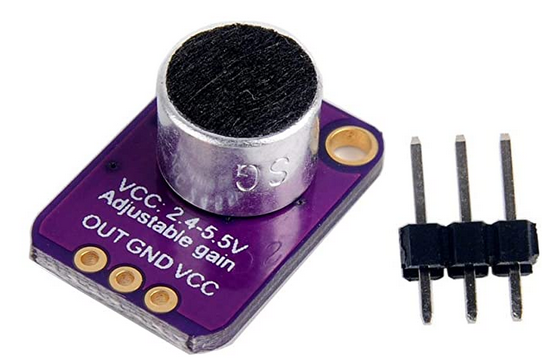
\includegraphics[width = 0.2\linewidth]{micBoard}
	\caption{The Audio board in Plan}
	\label{fig:audioboard}
\end{figure}
\begin{figure}
	\centering
	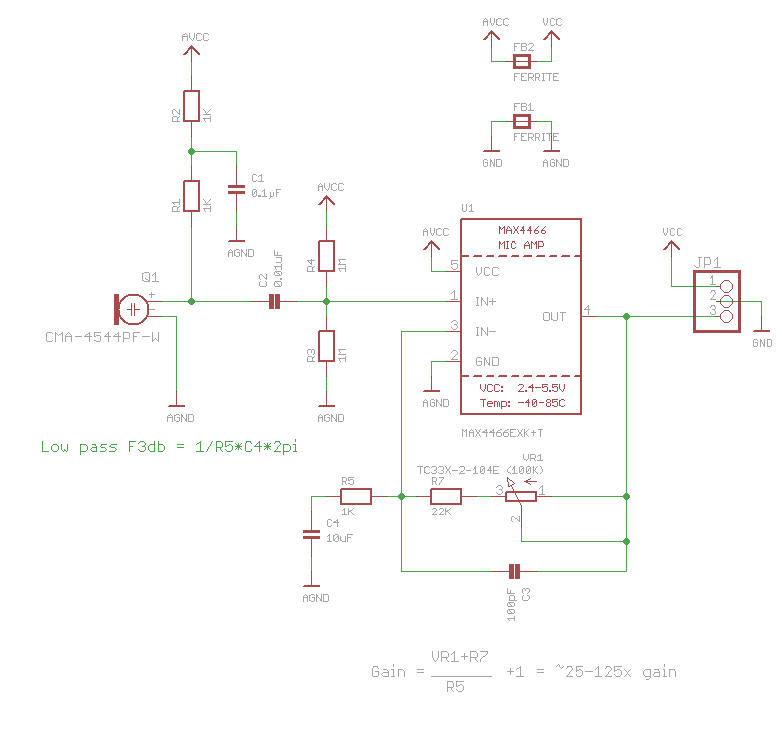
\includegraphics[width = 0.8\linewidth]{audioscem}
	\caption{Microphone Board Schematic}
	\label{fig:audioscem}
\end{figure}

\subsection*{Inputs and Outputs}
The input to the buzzer system is a Boolean value from he main code to trigger the buzzer.
As well the input to the microphone is the sound of the phone alarm to the microphone creating the signal for detection.
The system output is a PWM signal to power the buzzer to output sounds.
The microphone sensor output is a signal that needs to be read by the MCU's ADC.
 
\subsection*{Parameters}
The main parameter is the value for calibrating if the audio sensor has heard the phone ringing alarm.
The second parameter is then the Boolean value to provide to the main MCU code as input.
The third value is the duty cycle which controls the buzzer.  

\subsection*{Development Plan}
The plan is to develop the buzzer first as its simpler while I am focused on bed detection and main code functions. 
Only later will I test the microphone since it is a lower deterministic function and the device will still mainly function without it.
This is mentioned in section \ref{sec:risky} where I discuss the risks.\\

The plan:
\begin{itemize}
	\item Connect buzzer and check it's sound and adjust pwm input
	\item Connect microphone and create MCU code to read its values
	\item Determine if microphone can distinguish the alarm should from normal background noise 
	\item Record calibration value
\end{itemize}

\subsection*{Test Plan}
The test plan for the buzzer is simple, see if the sound is outputted and is heard well enough. 
For the microphone I want to test various phone alarm tones to check it can detect them and detain how close or far away to the microphone I need to be in order to trigger my code. 

\section{Most Critical Module}
The most critical and deterministic function is the bed occupancy detection since without it the whole thing wont work.
For this reason I have outlined two solutions for the detection system.
I have already preformed preliminary tests on the half bridge concept by disassembling a bathroom scale and placing on of its sensors under a leg of my bed, seen in figure \ref{fig:preliminary}. 
The scale displayed two different values when the bed was empty and occupied. 
This proves that this method would function once it is properly implemented though implementation could be tricky. 
There is no preliminary test I can do for the FSR before purchasing it and testing it as outlines in its development plan.\\


\section{Risk and Countermeasures} \label{sec:risky}
The biggest risk is not getting the bed detection to work which is the most critical function. 
Because of its complexity it could be time heavy as well and therefore I will prioritize this function over the rest which could cause the other functions to be incomplete. 
I have two methods for this function as a countermeasure if one doesn't work. 
If I am not able to get the bed detection to work on the bed I will try to show a proof of concept solution. 
This could be making it into a chair occupancy instead which is a more rigid structure and has a smaller scale than the bed.  \\

Another risk is the sound sensor not being sensitive enough and wont distinguish between an alarm or someone yelling in the room.
Finally a big risk is not being able to implement all functions in time. 
I am open to the possibility if I ran out of time to not complete the audio sensor as it's a simpler function and the device still work with a button to begin its functionality instead.
All it will mean for the user, is that they turn the device on instead of it being related to the phone.  
I will try to start my main two functions early for this risk. 
As well due to the at home situation, if something need to be purchased it could take longer to arrive or I will be delayed if I need to get emplacements for sensors.
There is no avoiding this risk except purchasing the sensors early to make sure i have time to exchange if they wont work and have enough time for shipping.

\section{Learning Objectives}
By preforming this project I will work on my MCU coding skills by creating a flow of code functions.
I will use timer functionality, and ADC functionality as well as general ISR and IOs.
I will learn about audio signals from the volume sensor and buzzer. 
Finally I will gain experience using Wheatstone bridge for strain gauges sensors and learning about their uses. 

\end{document}